\documentclass[a4paper,12pt,openany]{memoir}

%\usepackage{xltxtra}
%\defaultfontfeatures{Scale=MatchLowercase,Mapping=tex-text}
\usepackage{charter}
%\usepackage[urw-garamond]{mathdesign}
%\usepackage[bitstream-charter]{mathdesign}
%\usepackage[tpagella]{mathdesign}
%\usepackage{ucs}
%\usepackage[utf8x]{inputenc}  % adding the UTF-8 encoding
%\usepackage{culmus}
%\usepackage[HE8,OT1]{fontenc}
%\usepackage[english,hebrew]{babel}
\usepackage{setspace}
\usepackage{multicol}

\usepackage{polyglossia}
\usepackage{fontspec}

\setdefaultlanguage{english}

\setotherlanguage[numerals=hebrew]{hebrew}

\fontspec [Path = /Users/scott/Library/Fonts/culmus-0.132/ ,UprightFont = *Regular,  BoldFont      = *Demi-Bold]{Shofar}

\newfontfamily\hebrewfont[Script=Hebrew]{Shofar}

\setlength{\beforechapskip}{0cm}


\newenvironment{HgHebrew}{\begin{hebrew}\strut\\\noindent\Large}{\end{hebrew}}
\newcommand{\HgHL}[1]{{\large\textbf{#1}\par\noindent\\[-.5em]}}
\newcommand{\HgFill}{\vfill \hrule \vfill}

\newenvironment{HgEnglish}{\strut\\\noindent}{\vspace{1em}}
\newenvironment{HgTranslit}{\strut\\\noindent\begin{itshape}}{\end{itshape}\vspace{1em}}
\newcommand{\HgInst}[1]{{\noindent\sffamily{\bfseries{#1}}}}
\newcommand{\LSrc}{\textsuperscript{\upshape{[L]}}}

\newenvironment{myitemize}[0]{%
        \protect\begin{itemize}%
        \vspace*{-2mm}%
        \setlength{\topsep}{-6pt}%
        \setlength{\labelsep}{4pt}%
        \setlength{\partopsep}{-6pt}%
        \setlength{\itemsep}{-2pt}}%
{\protect\end{itemize}}


\newenvironment{myenumerate}[0]{%
        \protect\begin{enumerate}%
        \vspace*{-2mm}%
        \setlength{\topsep}{-6pt}%
        \setlength{\labelsep}{4pt}%
        \setlength{\partopsep}{-6pt}%
        \setlength{\itemsep}{-2pt}}%
{\protect\end{enumerate}}

\title{Haggadah}
\author{Seder for the perplexed family}

\begin{document}
\maketitle

\chapter*{The Passover seder}

\vfill

\vspace{-2em}
\begin{HgHebrew}
  \begin{center}
  קדש 
  -
  ורחץ
  -
  כרפס 
  -
  יחץ 
  -
  מגיד 
  -
  רחצה 
  -
  מוציא
  -
  מצה 
  \\
  מרור 
  -
  כורך 
  -
  שולחן עורך 
  -
  צפון
  -
  ברך 
  -
  הלל 
  -
  נירצה 
  \end{center}
\end{HgHebrew}
\vspace{-3em}
\begin{HgTranslit}
  \begin{center}
  {\small 
    KADESH - UR\d{H}ATZ - KARPAS - YA\d{H}ATZ - % \\
    MAGID - RA\d{H}TZA - MOTZI - MATZAH \\ 
    MAROR - KOREI\d{H} - SHUL\d{H}AN OREI\d{H} - % \\
    TZAFUN - BAREI\d{H} - HALLEL - NIRTZAH}
  \end{center}
\end{HgTranslit}


\newpage

\section*{Kiddush}

\noindent
On Shabbat

\begin{tabular}{r}
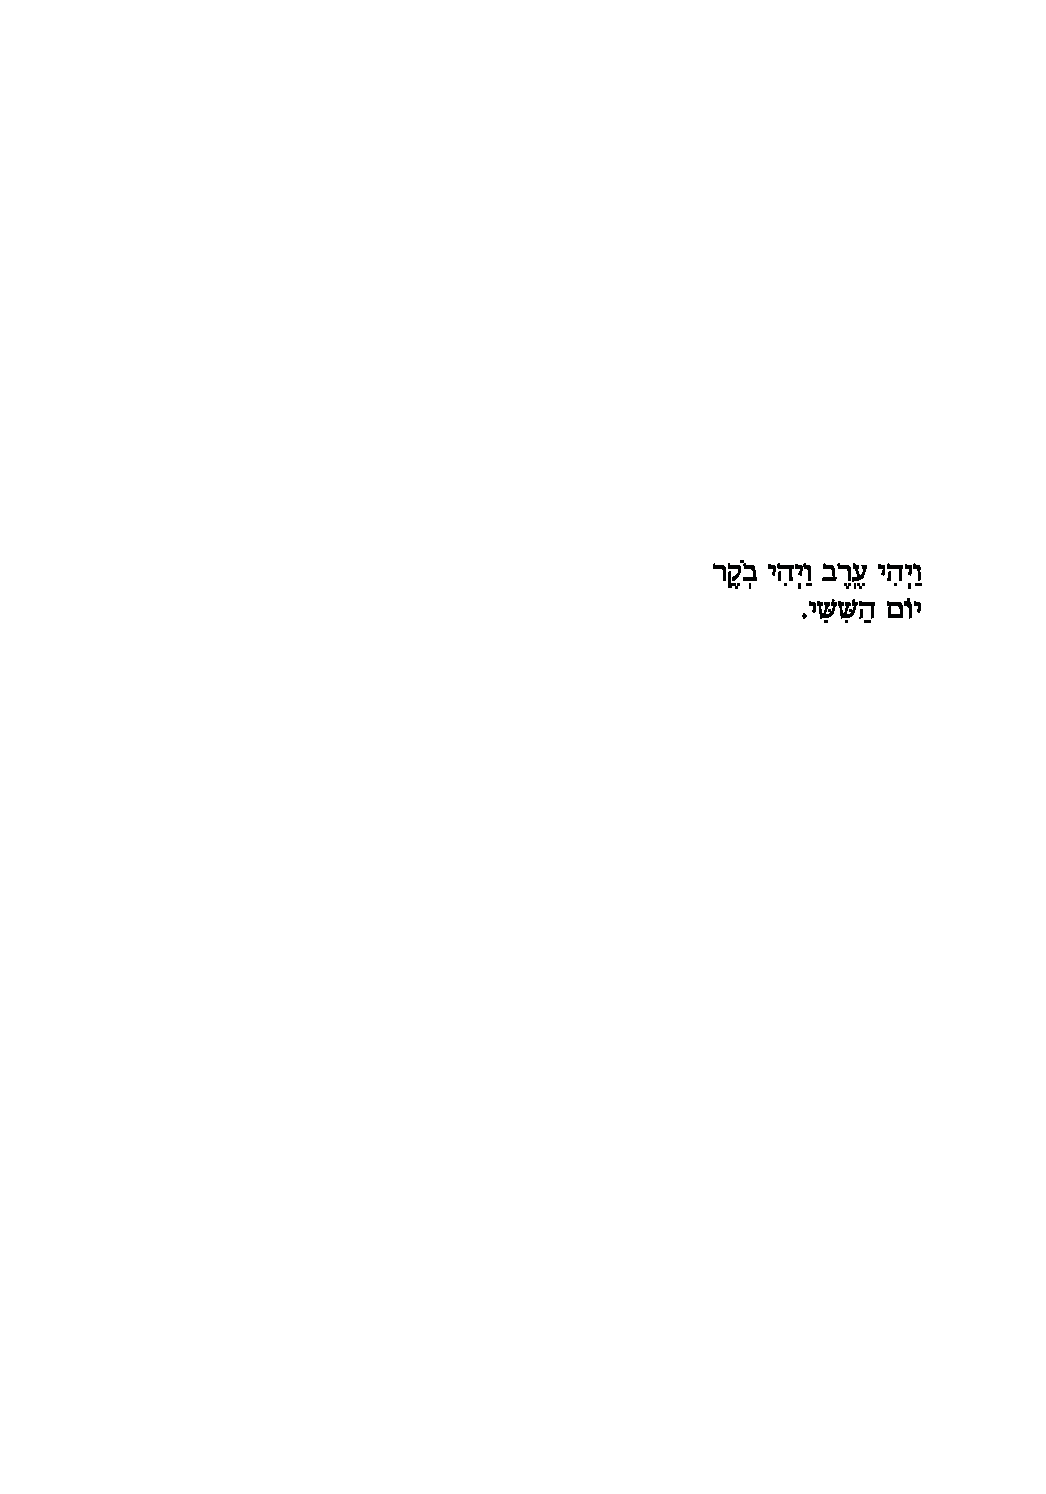
\includegraphics[width=6cm]{figs/0A010-vayehi}\\
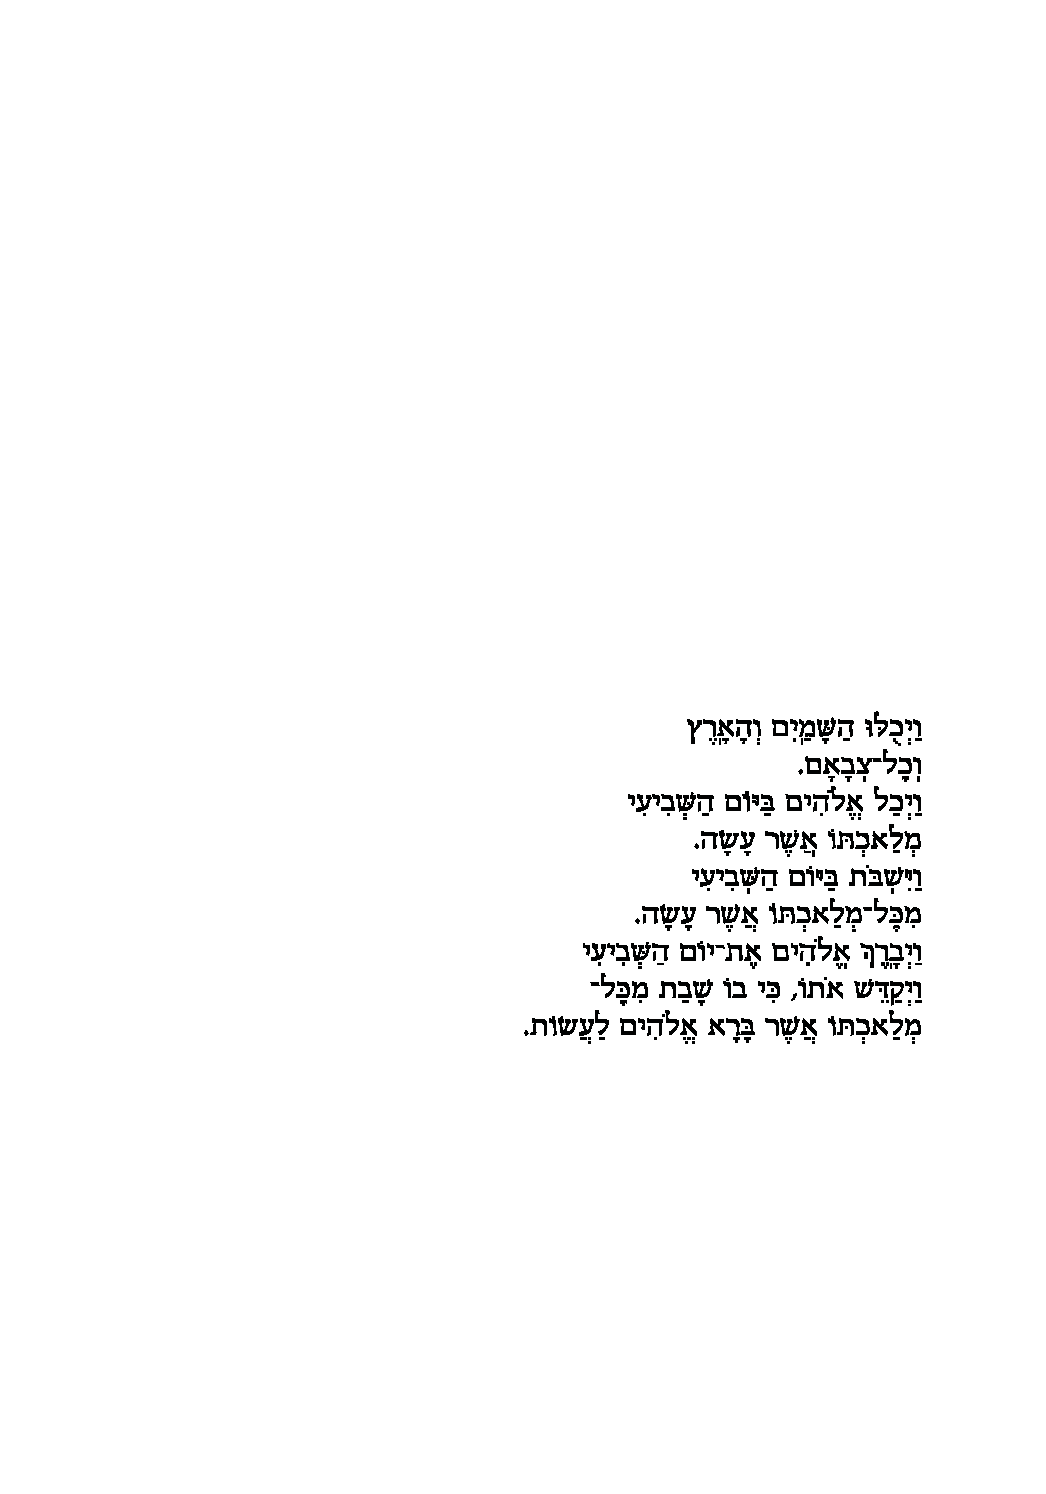
\includegraphics[scale=1.5,trim=0mm 0mm 2mm 0mm,clip]{figs/0A014-vayechulu}\\
\end{tabular}


\newpage
\HgInst{Pour the first cup of wine, and read:}

\begin{tabular}{r}
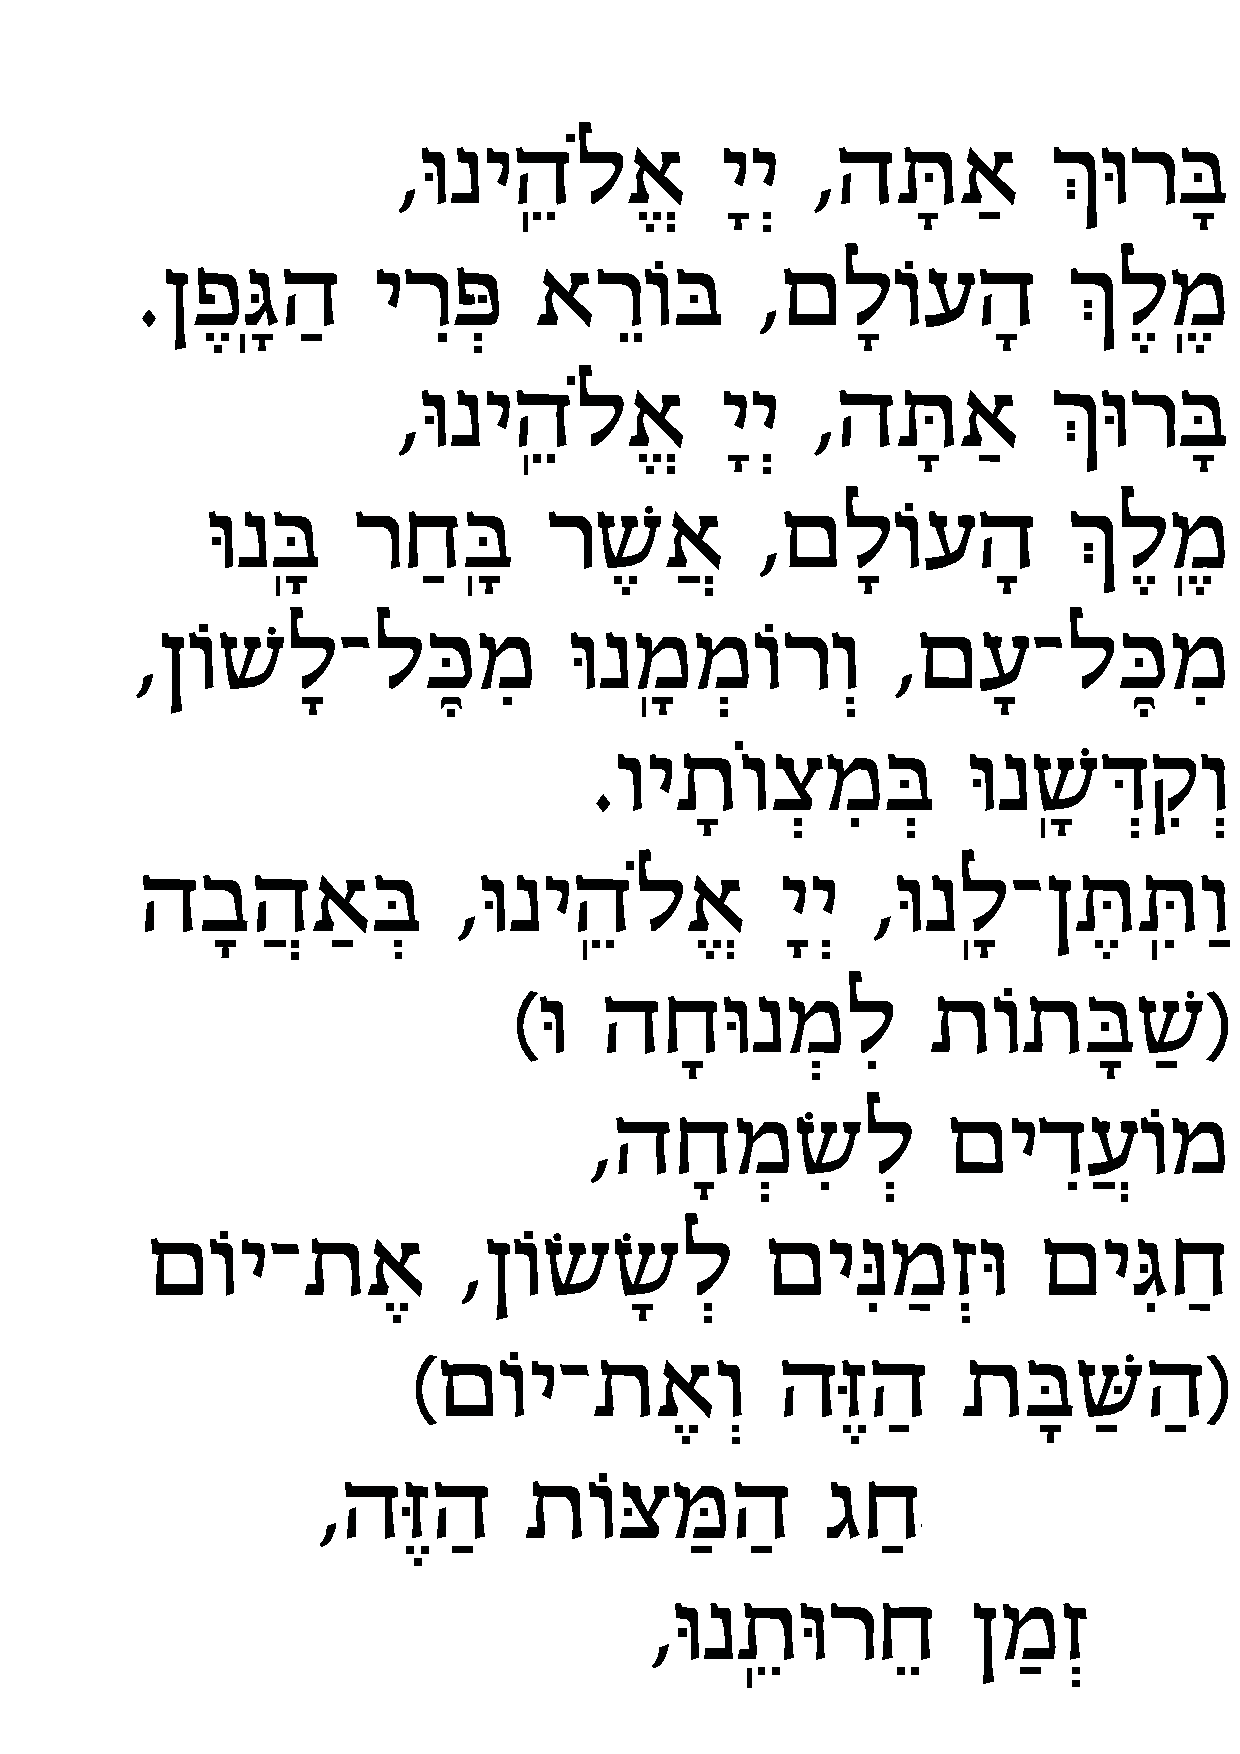
\includegraphics[width=9cm]{figs/0A020-kiddush1}\\
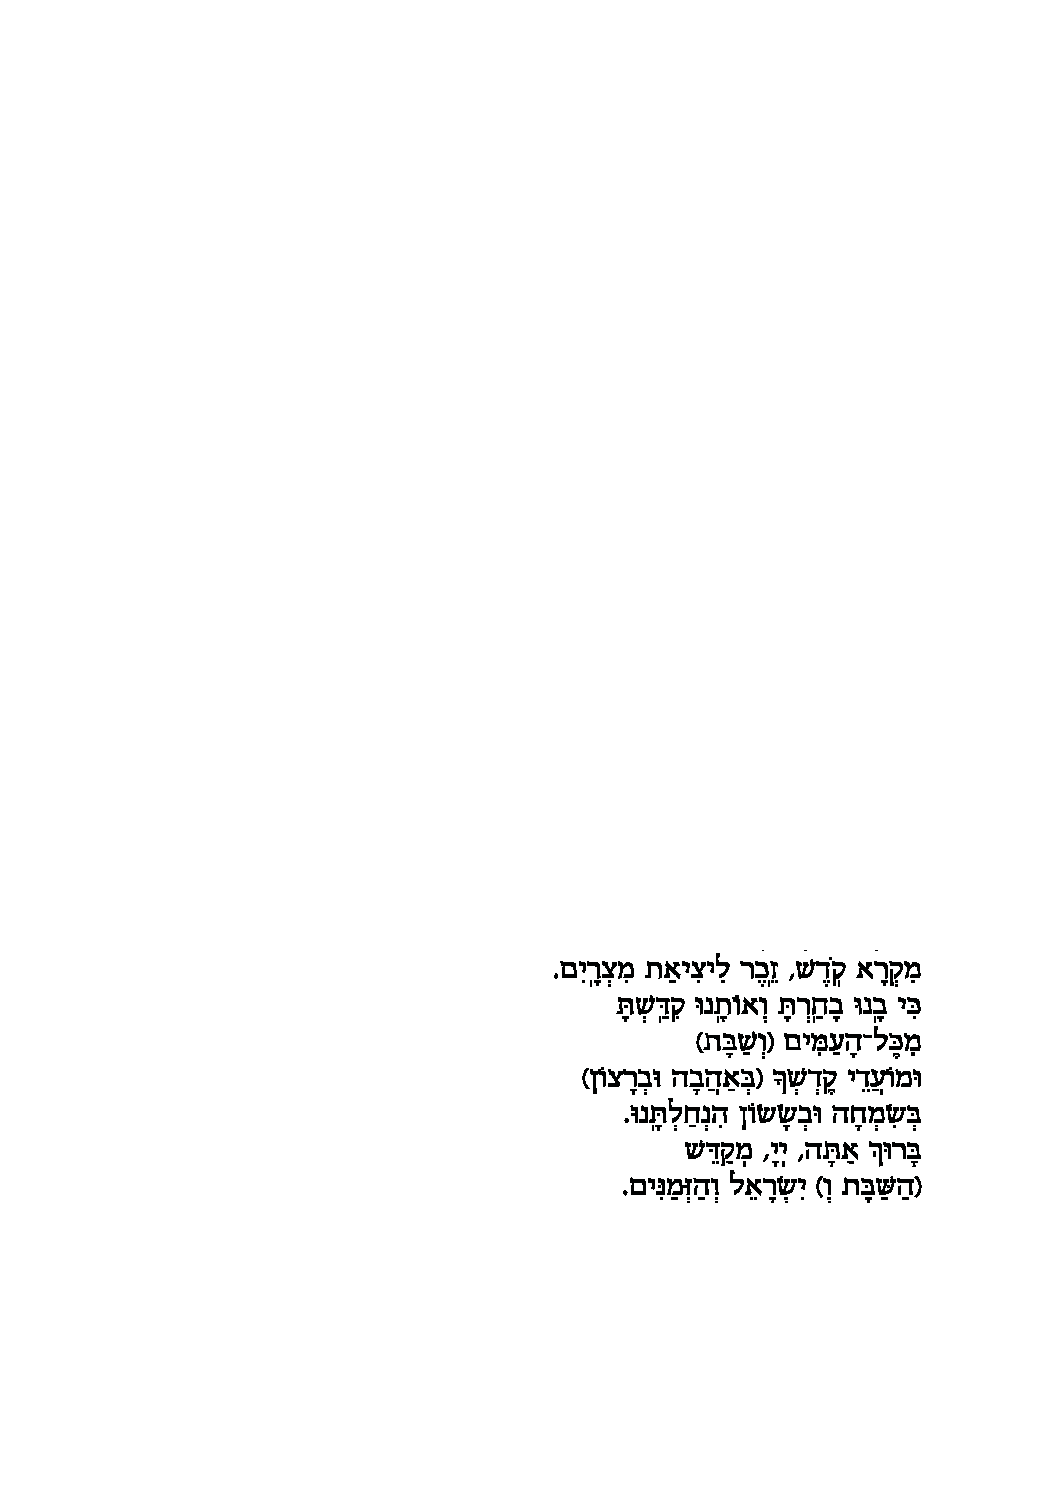
\includegraphics[width=9cm]{figs/0A024-kiddush2}\\
\end{tabular}


\newpage
\paragraph*{Shehecheyanu}

\begin{HgHebrew}
 בָּרוּךְ אַתָּה אֲדֹנָי אֱלֹהֵינוּ מֶלֶךְ הָעוֹלָם,
 שֶׁהֶחֱיָנוּ וְקִיְּמָנוּ וְהִגִּיעָנוּ לַזְּמָן הַזֶּה.
\end{HgHebrew}


\begin{HgTranslit}
Baruch atah Adonai, Eloheinu Melech haolam,
shehecheyanu, v'kiy'manu, v'higianu laz'man hazeh.
\end{HgTranslit}

\begin{HgEnglish}
Our praise to You, Eternal our God, Sovereign of all:
for giving us life, sustaining us, and enabling us to reach this season.
\end{HgEnglish}

\noindent
\HgInst{Drink the first cup of wine}

\vfill


\section*{Ur\d{h}atz: Washing the hands}


\HgInst{Those who wish to may wash your hands, without reciting a blessing.}


\vfill

\newpage

\section*{Karpas: The green vegetable}

\begin{HgEnglish}
  The green vegetable represents rebirth, renewal and growth. The salt
  water represents the tears we shed when we were slaves in Egypt. The
  karpas is usually a fresh vegetable like parsley, watercress or
  celery, though there are other cusoms.
\end{HgEnglish}

\vfill

\HgInst{Distribute the karpas, and dip them in saltwater.}

\begin{HgHebrew}
  בָּרוּךְ אַתָּה יי אֱלֹהֵינוּ מֶלֶךְ הָעוֹלָם, 
  \\
  בּוֹרֵא פְּרִי הָאֲדָמָה.

%ברוך אתה יי אלהינו מלך העולם, 
%  \\
%  בורא פרי האדמה.
\end{HgHebrew}

\begin{HgTranslit}
  Baru\d{h} atah Adonai, eloheinu mele\d{h} ha'olam, \\
  borei p'ri ha'adamah.
\end{HgTranslit}
\vspace{-1em}
\begin{HgEnglish}
  Blessed are you, Lord our God, ruler of the universe, \\
  Who creates the fruit of the earth.
\end{HgEnglish}

\HgInst{Eat the karpas.}

\vfill

\newpage
\section*{ Ya\d{h}atz: Breaking the matzah}
\vfill

\HgInst{Break the middle matzah, and set aside the larger piece as the
afikoman. Hold the remaining matzah up, and read:}

\begin{HgEnglish}
  \HgHL{
  This is the bread of affliction that our ancestors ate \\
  in the land of Egypt.
  }
  All who are hungry, come and eat; \\
  all who are needy, come and celebrate the Passover. \\
  Now we are here;
  next year may we be in Israel; \\
  now we are slaves;
  next year may we be free.
\end{HgEnglish}

\begin{HgHebrew}
  הָא לַחְמָא עַנְיָא דִּי אֲכָלוּ אַבְהָתָנָא
  \\
  בְּאַרְעָא דְמִצְרָיִם.
  \\
  כָּל דִּכְפִין יֵיתֵי וְיֵכוֹל,
  \\
  כָּל דִּצְרִיךְ יֵיתֵי וְיִפְסַח. 
  \\
  הָשַּׁתָּא הָכָא,
  לְשָׁנָה הַבָּאָה בְּאַרְעָא דְיִשְׂרָאֵל.
  \\
  הָשַּׁתָּא עַבְדֵי,
  לְשָׁנָה הַבָּאָה בְּנֵי חוֹרִין.
\end{HgHebrew}

\begin{HgTranslit}
  Hala\d{h}ma anya di a\d{h}alu avhatana \\
  b'ara d'mitzrayim.
  Kol di\d{h}fin yeitei v'ye\d{h}ol \\
  kol ditzri\d{h} yeitei v'yifsa\d{h}. \\
  Hashata ha\d{h}a, %\\
  l'shanah haba'ah b'ara d'yisrael. \\
  Hashata avdei, %\\
  l'shanah haba'ah b'nei \d{h}orin.
\end{HgTranslit}


\vfill

\HgInst{Pour (but not drink!) the second cup of wine.}

\vfill

\newpage

\section*{Magid: The Passover story \\ {The four questions}}

\vfill

\HgInst{The youngest person present  (however defined, or next in
  turn) recites:}

\begin{HgEnglish}
  \HgHL{Why is this night different from all other nights?}
  On other nights, we eat leavened bread and matzah; tonight only matzah. \\
  On other nights, we eat all kinds of herbs; tonight bitter herbs. \\
  On other nights, we do not dip our food; tonight we dip twice. \\
  On other nights, we eat upright or reclining; tonight we all recline. \\
\end{HgEnglish}

\begin{HgHebrew}
מַה נִּשְּׁתַּנָה הַלַּיְלָה הַזֶּה מִכָּל הַלֵּילוֹת? 
\\
שֶׁבְּכָל הַלֵּילוֹת אָנוּ אוֹכְלִין חָמֵץ וּמַצָּה,
%\\
הַלַּיְלָה הַזֶּה כּוּלוֹ מַצָּה. 
\\
שֶׁבְּכָל הַלֵּילוֹת אָנוּ אוֹכְלִין שְׁאָר יְרָקוֹת,
%\\
הַלַּיְלָה הַזֶּה מָרוֹר. 
\\
שֶׁבְּכָל הַלֵּילוֹת אֵין אֶנוּ מַטְבִּילִין אֲפִילוּ פַּעַם אֶחָת, 
%\\
הַלַּיְלָה הַזֶּה שְׁתֵּי פְעָמִים. 
\\
שֶׁבְּכָל הַלֵּילוֹת אָנוּ אוֹכְלִין בֵּין יוֹשְׁבִין וּבֵין מְסֻבִּין, 
%\\
הַלַּיְלָה הַזֶּה כֻּלָנו מְסֻבִּין. 
\end{HgHebrew}

\begin{HgTranslit}
  \HgHL{Ma nishtanah halailah hazeh mikol haleilot?}
  Shebe\d{h}ol haleilot, anu o\d{h}lin \d{h}ametz umatzah, 
  halailah hazeh kulo matzah. \\
  Shebe\d{h}ol haleilot, anu o\d{h}lin sh'ar y'rakot, 
  halailah hazeh maror. \\
  Shebe\d{h}ol haleilot, ein anu matbilin afilu p'am e\d{h}ad,
  halailah hazeh sh'tei f'amin. \\
  Shebe\d{h}ol haleilot, anu o\d{h}lin bein yoshvin uvein m'subin,
  halailah hazeh \\ \strut $\quad$ kulanu m'subin.
\end{HgTranslit}

\newpage

\HgInst{Uncover the matzah, and read:}

\begin{HgEnglish}
We were slaves of Pharaoh in Egypt, and our God brought us out from there
with a mighty hand and an outstretched arm.
Now, if God had not brought our ancestors out from Egypt, then we, our
children, and our children's children might still be enslaved to Pharaoh in
Egypt.  Therefore, even if we were all wise, all understanding, all learned in
the ways of Torah, we would still be obligated to tell the story of the Exodus.
And indeed, everyone who dwells upon the features of the Exodus is
praiseworthy.

%It happened that Rabbi Eliezer, Rabbi Yehoshua, Rabbi Elazar ben Azaryah, Rabbi
%Akiva and Rabbi Tarphon were reclining [at a seder] in B'nei Berak. They were
%discussing the exodus from Egypt all that night, until their students came and
%told them: ``Masters! The time has come for reciting the morning Sh'ma!''
Rabbi Eleazar ben Azariah said: I have lived to be a man of threescore years and
ten, yet I did not understand why the story of the Exodus should be told at
night until Ben Zoma explained it to me. He said: It is said, ``That thou mayest
remember the day when thou camest forth out of the land of Egypt all the days of
thy life.'' (Deuteronomy 16:3) ``The days of your life'' would have meant the
days only, but ``all the days of your life'' includes the nights also.  The
Sages of Israel explain it further: ``The days of your life'' refers to this
world, while ``All the days of your life'' includes the time of the Messiah.

\end{HgEnglish}

\HgInst{Continue}

\begin{HgEnglish}
The Torah speaks of four kinds of children: The wise child, the wicked
child, the simple child, and the child who does not know how to ask.
\begin{myitemize}
\item The wise child asks: ``What is the meaning of the testimonies, laws and
judgments which God has commanded you?''\\
To that one, you explain all the laws of Passover, down to the very last detail
about the Afikoman

\item  The wicked child asks: ``What does all of this mean to you?'' (Exodus
12:26). By saying ``you,'' and not ``we'' or ``me,'' he excludes himself from the group,
and denies God. 

Answer plainly: ``This is done because of what the
Lord did for me when I came out of Egypt.'' ``For me, not for you:
if you had been there in Egypt, you would not have been redeemed.''

\item The simple child asks: ``What is this?'' 

Answer that one: ``By strength of hand the Lord brought us out from Egypt, from
the house of bondage.'' 

\item To the child who does not know how to ask, speak first, it is written: ``And
thou shalt show thy son in that day, saying, This is done because of that which
the Lord did unto me when I came forth out of Egypt.'' 
\end{myitemize}
\end{HgEnglish}

\HgInst{Continue}

\begin{HgEnglish}
My father was a wandering Aramean. He went down to Egypt sojourned
there in small numbers, and became a large, mighty and populous
nation. They said to Pharaoh, we have come to sojourn in the land, for
there is no pasture for your servants' flocks because the hunger is
severe in the land of Canaan; and now, please, let your servants dwell
in the land of Goshen.

The Egyptians treated us badly and they made us suffer, and they put hard work upon us.

The Egyptians treated us badly, as it is said: Come, let us act cunningly with [the people] lest they multiply and, if there should be a war against us, they will join our enemies, fight against us and leave the land."

"And they made us suffer," as it is said: "They set taskmasters over [the people of Israel] to make them suffer with their burdens, and they built storage cities for Pharaoh, Pitom and Ramses."

"And they put hard work upon us," as it is said: "The Egyptians made the children of Israel work with rigor. And they made their lives bitter with hard work, with mortar and with bricks and all manner of service in the field, all their work which they made them work with rigor."

And we cried out to Adonai, the God of our fathers, and Adonai heard
our voice and saw our suffering, our labor and our oppression, and
remembered His covenant with Abraham, Isaac and Jacob.

The L-rd took as out of Egypt with a strong hand and an outstretched arm, and with a great manifestation, and with signs and wonders."

"The L-rd took us out of Egypt," not through an angel, not through a seraph and not through a messenger. The Holy One, blessed be He, did it in His glory by Himself!

Thus it is said: "In that night I will pass through the land of Egypt, and I will smite every first-born in the land of Egypt, from man to beast, and I will carry out judgments against all the gods of Egypt, I the L-rd."

"I will pass through the land of Egypt," I and not an angel;

"And I will smite every first-born in the land of Egypt," I and not a seraph;

"And I will carry out judgments against all the gods of Egypt," I and not a messenger;

"I- the L-rd," it is I, and none other!

"With a strong hand," this refers to the dever (pestilence) as it is said: "Behold, the hand of the L-rd will be upon your livestock in the field, upon the horses, the donkeys, the camels, the herds and the flocks, a very severe pestilence."

"And with an outstretched arm," this refers to the sword, as it is said: "His sword was drawn, in his hand, stretched out over Jerusalem."

"And with a great manifestation," this refers to the revelation of the Shechinah (Divine Presence), as it is said: "Has any G‑d ever tried to take for himself a nation from the midst of another nation, with trials, signs and wonders, with war and with a strong hand and an outstretched arm, and with great manifestations, like all that the L-rd your G‑d, did for you in Egypt before your eyes!"

"And with signs," this refers to the staff, as it is said: "Take into your hand this staff with which you shall perform the signs."

"And wonders," this refers to the blood, as it is said: "And I shall show wonders in heaven and on earth.
\end{HgEnglish}

% \begin{HgEnglish}
% Wise, wicked, simple, does not know how to ask. This order conforms neither to
% the order in which the children are mentioned in the Torah (Wicked, Simple, Does
% Not Know How to Ask, Wise), nor to the order of their moral standing, in which
% the wicked child should be last.

% Rather, they are listed in order of their intellectual capacities: The wise
% child; the wicked child, who is also wise but whose insolence leads him to act
% wickedly; the simple child, who has at least enough intelligence to ask; and
% finally the one who does not know how to ask

% \HgSource{Chabad}
% \end{HgEnglish}



\end{document}

%%% Local Variables: 
%%% mode: latex
%%% TeX-master: t
%%% End: 
